% small.tex
\documentclass{beamer}
\usepackage{fancyvrb}
\usepackage{color}
\usepackage{hyperref}
\hypersetup{
  colorlinks = false,
  urlcolor = blue,
  pdfauthor = {Alexander Mazurov},
  pdfkeywords = {scientific computing, system and distributing programming},
  pdftitle = {Optimization of software trigger and chi_b studies in LHCb}
  pdfsubject = {Optimization of software trigger and chi_b studies in LHCb},
  pdfpagemode = UseNone
}
% ============================================================================
\title{Optimization of software trigger and $\chi_b$ studies in LHCb}
\subtitle{2nd year report}
\institute[University of Ferrara]{
  Department of Physics\\
  University of Ferrara, Italy\\
  \&\\
  LHCb experiment, CERN, Switzerland\\
  \texttt{alexander.mazurov@cern.ch}
}
% ============================================================================
\author{Alexander (Sasha) Mazurov}
\date{30 November 2012}
\usetheme{Copenhagen}
% ============================================================================
\begin{document}

\maketitle
\section{Introduction}
% ============================================================================
\begin{frame}
% ----------------------------------------------------------------------------
\frametitle{About Me}
\begin{columns}[c]
\column{60mm}
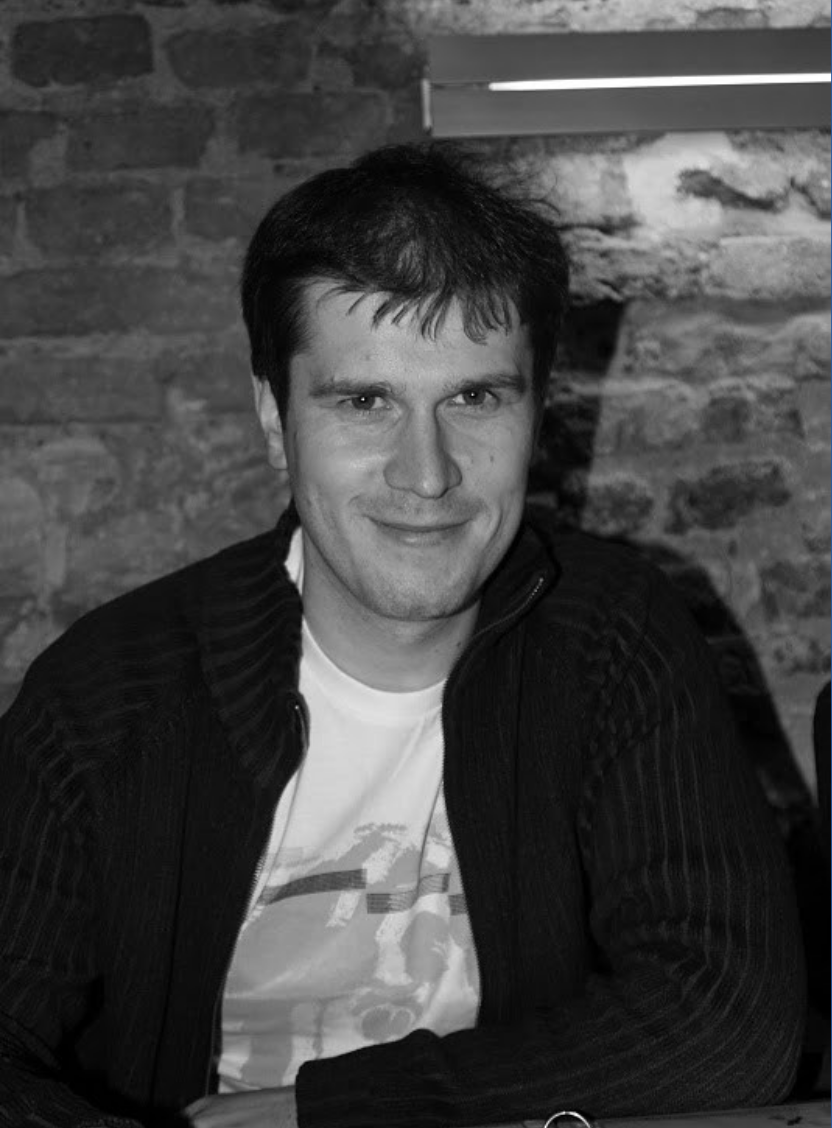
\includegraphics[width=60mm]{images/me.png}
\column{60mm}
\begin{itemize}
    \item {\bf 1997-2002:} Lomonosov's Moscow State University, MS Calculate
    Mathematic and System programming.
    \item {\bf 2005-present:} CERN, LHCb experiment.
\end{itemize}
\end{columns}
% ----------------------------------------------------------------------------
\end{frame}
% ============================================================================
\begin{frame}
% ----------------------------------------------------------------------------
\frametitle{LHCb experiment (1)}
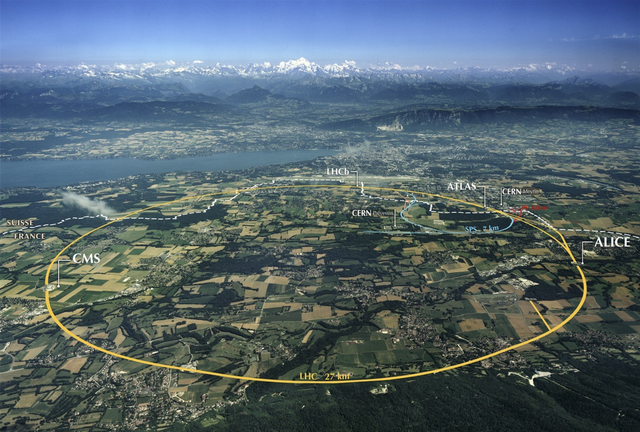
\includegraphics[width=100mm]{images/lhcb.png}
% ----------------------------------------------------------------------------
\end{frame}
% ============================================================================
\begin{frame}
% ----------------------------------------------------------------------------
\frametitle{LHCb experiment (2)}
Core physics program is in the study of processes with hadrons formed by b-
and c-quarks:
\begin{itemize}
    \item B-mesons
    \item D-mesons
\end{itemize}

\begin{alertblock}{Hot result (November 2012)}
First evidence for the $B^{0}_{s} \rightarrow \mu \mu$ decay.
\end{alertblock}
% ----------------------------------------------------------------------------
\end{frame}
% ============================================================================
\begin{frame}
% ----------------------------------------------------------------------------
\frametitle{My research activities}
\begin{enumerate}
    \item Trigger software profiling. \textcolor{green}{DONE}
    \item Study of $\chi_{b}$ decays. \textcolor{blue}{IN PROGRESS}
\end{enumerate}
% ----------------------------------------------------------------------------
\end{frame}
% ============================================================================
\section{Trigger software profiling}
\begin{frame}
\begin{exampleblock}{}
  \begin{center}
    {\huge Trigger software profiling}
  \end{center}
\end{exampleblock}

\end{frame}

\begin{frame}
\frametitle{Trigger software profiling}
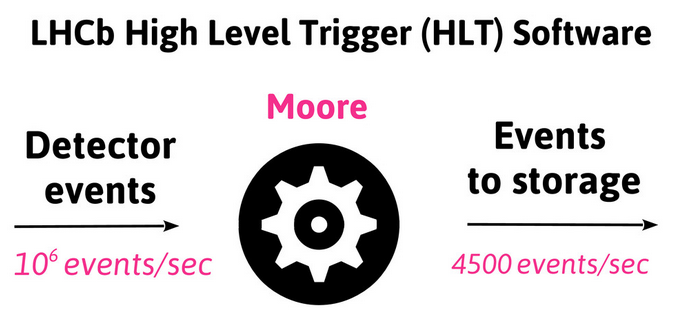
\includegraphics[width=100mm]{images/moore.png}
\end{frame}
\subsection{Profiler Auditor}
\begin{frame}
\frametitle{CPU Profiler Auditor}
\begin{columns}[c]
\column{.5\textwidth}
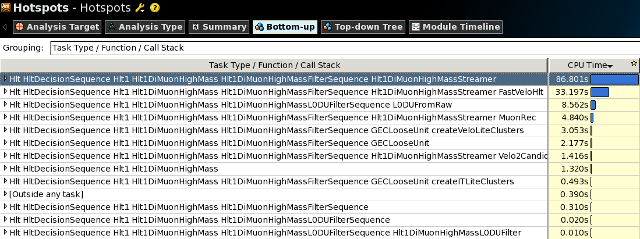
\includegraphics[width=\textwidth]{images/cpu01.png}\\~\\
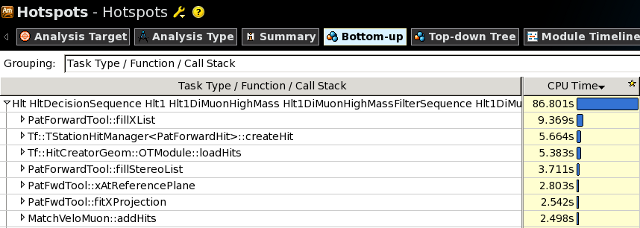
\includegraphics[width=\textwidth]{images/cpu02.png}
\column{.5\textwidth}
\begin{itemize}
    \item C++ library.
    \item Deployed into the core software framework in LHCb --- Gaudi.
    \item Based on Intel\textsuperscript{\textregistered} VTune\texttrademark
    Amplifier XE User API
\end{itemize}
\end{columns}
\end{frame}

\begin{frame}
\frametitle{Main Features}
\begin{itemize}
    \item Group results by dynamic properties of the program: names of algorithms.
    \item Show CPU usage by source line.
\end{itemize}
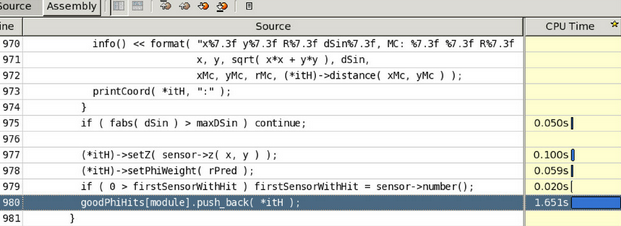
\includegraphics[width=\textwidth]{images/cpu03.png}
\end{frame}

\begin{frame}
\frametitle{Trigger profiling}
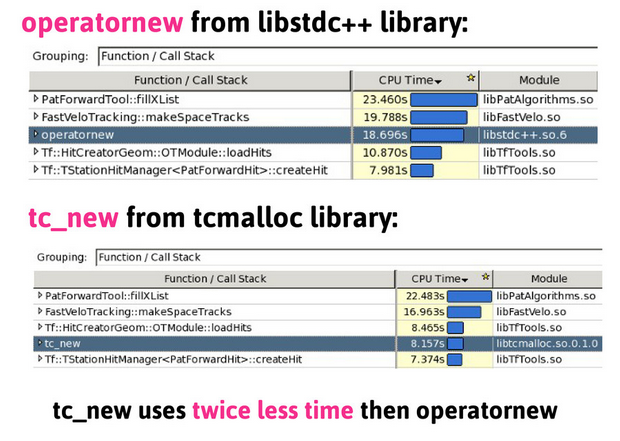
\includegraphics[width=\textwidth]{images/hlt.png}
\end{frame}
\begin{frame}
\frametitle{CHEP2012: Talk and Paper}
\begin{columns}[c]
\column{.5\textwidth}
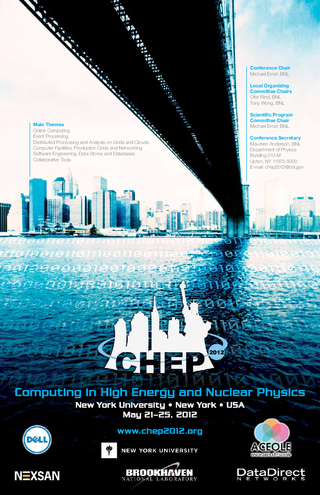
\includegraphics[width=45mm]{images/chep.png}
\column{.5\textwidth}
\begin{itemize}
    \item Paper "Advanced Modular Software Performance Monitoring", Journal of Physics: Conference Series
    \item \href{http://cern.ch/go/w6C8}{http://cern.ch/go/w6C8}
\end{itemize}
\end{columns}
\end{frame}
\section{Study of $\chi_{b}$ decays.}
\begin{frame}
\begin{exampleblock}{}
    \begin{center}
        {\huge Study of $\chi_{b}$ decays}
    \end{center}
\end{exampleblock}
\end{frame}
\begin{frame}
\frametitle{Plan}
\begin{enumerate}
  \item Measurement for $\Upsilon(NS)$ (N=1, 2, 3) cross sections in $\chi_b$ decays as a function of $p_T(N\Upsilon)$
  \item Measurement of $\chi_{b}(3P)$ mass.
\end{enumerate}
\end{frame}
\begin{frame}
\frametitle{Cross section}
\begin{enumerate}
  \item $\Upsilon(1S)$
    \begin{enumerate}
      \item $\frac{\sigma(\chi_b(1P) \rightarrow \Upsilon(1S))}{\sigma(\Upsilon(1S))}[p_T(\Upsilon(1S))]$
      \item $\frac{\sigma(\chi_b(2P) \rightarrow \Upsilon(1S))}{\sigma(\Upsilon(1S))}[p_T(\Upsilon(1S))]$
      \item $\frac{\sigma(\chi_b(3P) \rightarrow \Upsilon(1S))}{\sigma(\Upsilon(1S))}[p_T(\Upsilon(1S))]$
    \end{enumerate}
  \item $\Upsilon(2S)$
    \begin{enumerate}
      \item $\frac{\sigma(\chi_b(2P) \rightarrow \Upsilon(1S))}{\sigma(\Upsilon(1S))}[p_T(\Upsilon(2S))]$
      \item $\frac{\sigma(\chi_b(3P) \rightarrow \Upsilon(1S))}{\sigma(\Upsilon(1S))}[p_T(\Upsilon(2S))]$
    \end{enumerate}
\end{enumerate}
\end{frame}
\end{document}